\section{Appendix}

\subsection{Polyhedral partition of modes}

For an entire link with discrete state space indexed by $i = 1,...,n$, and state $\boldsymbol\rho^{t} = (\rho_{0},\rho_{1},...,\rho_{n},\rho_{n+1})$ a n+2 dimensional vector which describes the state of the link in the space $\mathcal{S} = [0,\rho_{j}]^{n+2}$, we present a whole description of the space of ''modes'' along it, partitioned in different polyhedra. We can note that the ghost cells are included. Since there is always the entry $\rho_{i}$ in common for successive pairs $(\rho_{i-1},\rho_{i})$ and $(\rho_{i},\rho_{i+1})$, a correlation propagates along the link, reducing the number of modes to a quantity smaller than $3^{n}$.


\subsubsection{H-representation of a polyhedron}\label{sec:polytope}

A convex polyhedron (or polytope) may be defined as an intersection of a finite number of half-spaces. Such definition is called a \textit{half-space representation} or \textit{H-representation}.

\noindent A closed half-space can be written as a linear inequality:

\begin{equation}
a_{1}x_{1} + a_{2}x_{2} + ... + a_{n}x_{n} \leq b
\label{eq:closedHalfSpace}
\end{equation}

\noindent where $n$ is the dimension of the space containing the polytope under consideration. Hence, a \textit{convex polytope} may be regarded as the set of solutions to the system of linear inequalities:

\begin{equation}
\begin{array}{l}
a_{11}x_{1} + a_{12}x_{2} + ... + a_{1n}x_{n} \leq b_{1}\\
a_{21}x_{1} + a_{22}x_{2} + ... + a_{2n}x_{n} \leq b_{2}\\
...\\
a_{m1}x_{1} + a_{m2}x_{2} + ... + a_{mn}x_{n} \leq b_{m}
\end{array}
\label{eq:hRepresentation}
\end{equation}

\noindent where $m$ is the number of half-spaces defining the polytope (the dimension here is not related to the dimension of the space $\mathcal{S}$, and is used only for the definition). This can be concisely written as the matrix inequality:

\begin{equation}
Ax \leq b
\label{eq:matRepresentation}
\end{equation}

\noindent $A$ is an $m\times n$ matrix, $x$ is an $n\times 1$ column vector of variables, and $b$ is an $m\times 1$ column vector of constants. Here, we don't differentiate \textit{closed convex polyhedron} which are defined with large inequalities from \textit{open convex polyhedron} which are defined with strict inequalities. And the polyhedra $\textbf{W}_{i}, \textbf{L}_{i}, \textbf{D}_{i}$ defined in (\ref{eq:regions3}) for $i=0,...,n$ in the space $\mathcal{S}$ are represented with a mix of large and strict inequalities to have a proper partition of the space.


\subsubsection{Algorithm to find the minimal H-representation}\label{sec:minHrepresentation}

We use the indicator functions defined in (\ref{eq:indicators},\ref{eq:indicators2}). Starting from $i=0$, we evaluate $\alpha_{0}(\boldsymbol\rho)$, $\beta_{0}(\boldsymbol\rho)$, and $\gamma_{0}(\boldsymbol\rho)$ and get $s_{i}$, or equivalently $Q_{i}$, or the first two defining half-spaces of $\textbf{P}_{\boldsymbol s}$. By construction, the intersection of these two half-spaces are the \textit{minimal H-representation} of $Q_{0}$. Now suppose we have evalued the indicator functions and $s_{i}$ sequentially for $i=1,...,k$ and constructed the \textit{minimal H-representation} of $\bigcap_{i=0}^{k} \textbf{Q}_{i}$.

Case $s_{k}=w$: We have:

\begin{equation}
\begin{array}{l}
w_{k}(\boldsymbol\rho)=\alpha_{k}(\boldsymbol\rho)\gamma_{k}(\boldsymbol\rho)=1\\
\beta_{k+1}(\boldsymbol\rho)=\gamma_{k}(\boldsymbol\rho)=1\\
w_{k+1}(\boldsymbol\rho)=\alpha_{k+1}(\boldsymbol\rho)\gamma_{k+1}(\boldsymbol\rho)\\
l_{k+1}(\boldsymbol\rho)=1-\gamma_{k+1}(\boldsymbol\rho)\\
d_{k+1}(\boldsymbol\rho)=0
\end{array}
\end{equation}

\noindent This means that $s_{k+1}\in\{w,l\}$ and evaluating $\gamma_{k+1}(\boldsymbol\rho)$ suffices to find $s_{k+1}$. It is also necessary to evaluate $\gamma_{k+1}(\boldsymbol\rho)$ because its value is independent from the values of the indicator functions up to $i=k$ (given that $s_{k}=w$). Then $s_{k+1}$ is exactly determined by one of the two half-spaces $H_{\gamma_{k+1}}$ and $H^{d}_{\gamma_{k+1}}$, and adding one of them to the \textit{minimal H-representation} of $\bigcap_{i=0}^{k} \textbf{Q}_{i}$ gives the \textit{minimal H-representation} of $\bigcap_{i=0}^{k+1} \textbf{Q}_{i}$.

Case $s_{k}=l$: We have:

\begin{equation}
\begin{array}{l}
l_{k}(\boldsymbol\rho)=\beta_{k}(\boldsymbol\rho)(1-\gamma_{k}(\boldsymbol\rho))=1\\
\beta_{k+1}(\boldsymbol\rho)=\gamma_{k}(\boldsymbol\rho)=0\\
w_{k+1}(\boldsymbol\rho)=\alpha_{k+1}(\boldsymbol\rho)\gamma_{k+1}(\boldsymbol\rho)\\
l_{k+1}(\boldsymbol\rho)=0\\
d_{k+1}(\boldsymbol\rho)=1-\alpha_{k+1}(\boldsymbol\rho)
\end{array}
\end{equation}

\noindent A similar analysis shows that adding $H_{\alpha_{k+1}}$ or $H^{d}_{\alpha_{k+1}}$ gives the \textit{minimal H-representation} of $\bigcap_{i=0}^{k+1} \textbf{Q}_{i}$.

Case $s_{k}=d$: We have no prior information on $w_{k+1}(\boldsymbol\rho)$, $l_{k+1}(\boldsymbol\rho)$, and $d_{k+1}(\boldsymbol\rho)$ and have to evaluate each one of them to find the two defining half-spaces that give the \textit{minimal H-representation} of $\bigcap_{i=0}^{k+1} \textbf{Q}_{i}$, when added to the set of current defining half-spaces.

By recurrence, we have constructed a \emph{minimal H-representation} of $\textbf{P}_{\boldsymbol s}=\bigcap_{i=0}^{n} \textbf{Q}_{i}$, namely

\begin{equation}
\begin{array}{l}
\bigcap_{j=0}^{k} \textbf{H}_{j}\\
\textbf{H}_{j}\in \{\textbf{H}_{\alpha_{i}}, \textbf{H}^{d}_{\alpha_{i}}, \textbf{H}_{\beta_{i}}, \textbf{H}^{d}_{\beta_{i}}, \textbf{H}_{\gamma_{i}}, \textbf{H}^{d}_{\gamma_{i}}\}_{i=0,...,n}
\end{array}
\label{eq:minRepresentation}
\end{equation}

\noindent Hence, each of the defining half-spaces is of dimension $n+1$ \cite{Gruenbaum2003} (recall that the space $\mathcal{S} = [0,\rho_{j}]^{n+2}$ is of dimension $n+1$), and seperate by definition the polyhedron $\textbf{P}_{\boldsymbol s}$ from $(n+1)$-adjacent polyhedra $\textbf{P}_{\boldsymbol s'}$ of the polyhedral partition of $\mathcal{S}$.


\subsubsection{Proof of the exclusivity of all (n+1)-adjcacencies}\label{sec:adjacency}

Given a polyhedron $\textbf{P}_{\boldsymbol s}$ of the partition of $\mathcal{S}$, its minimal H-representation (\ref{eq:minRepresentation}) $\bigcap_{j=0}^{k} \textbf{H}_{j}$ given by the algorithm above, its H-representation $\bigcap_{i=0}^{n} \textbf{Q}_{i}$ given by (\ref{eq:Hrepresentation}, \ref{eq:Hrepresentation2}, \ref{eq:Hrepresentation3}), and an adjacent polyhedron $\textbf{P}_{\boldsymbol s'}$, there exists a unique $j\in\{0,...,k\}$ such that $\partial \textbf{H}_{j}$ ($=\bar{\textbf{H}}_{j} \backslash \textbf{H}^{0}_{j}$) is a common supportive hyperplane of $\textbf{P}_{\boldsymbol s}$ and $\textbf{P}_{\boldsymbol s'}$, by definition of the minimal H-representation. There exists $i'\in\{0,...,n\}$ such that

\begin{equation}
\begin{array}{l}
\textbf{Q}_{i'}=\textbf{H}_{j}\cap \textbf{H}_{i'}\\
\textbf{H}_{j}, \textbf{H}_{i'}\in \{\textbf{H}_{\alpha_{i'}}, \textbf{H}^{d}_{\alpha_{i'}}, \textbf{H}_{\beta_{i'}}, \textbf{H}^{d}_{\beta_{i'}}, \textbf{H}_{\gamma_{i'}}, \textbf{H}^{d}_{\gamma_{i'}}\}
\end{array}
\label{eq:adjacency1}
\end{equation}

\noindent and we can see from figure \ref{fig:godunovDiagram} that there exists $\textbf{R}_{i'}$ in $\{\textbf{W}_{i'}, \textbf{L}_{i'}, \textbf{D}_{i'}\}$ defined in (\ref{eq:regions3}) different from $\textbf{Q}_{i'}$ such that

\begin{equation}
\textbf{H}^{d}_{j}\cap \textbf{H}_{i'}\subset \textbf{R}_{i'}
\label{eq:adjacency2}
\end{equation}

\noindent Let $\mathcal{I}$ be the set of all $i'\in\{0,...,n\}$ such that we have (\ref{eq:adjacency1}, \ref{eq:adjacency2}), then $(\bigcap_{i\notin \mathcal{I}} \textbf{Q}_{i})\cap (\bigcap_{i'\in\mathcal{I}}\textbf{R}_{i'})$ is a polyhedron of the partition. Let us denote its associated mode $\boldsymbol s''$.

\begin{equation}
\begin{array}{ll}
\bar{\textbf{P}}_{\boldsymbol s}\cap \partial \textbf{H}_{j} & =(\bigcap_{i\notin \mathcal{I}} \bar{\textbf{Q}}_{i})\cap(\bigcap_{i'\in \mathcal{I}}\bar{\textbf{H}}_{i'})\cap\partial \textbf{H}_{j}\\
 & \subset (\bigcap_{i\notin \mathcal{I}} \bar{\textbf{Q}}_{i})\cap (\bigcap_{i'\in \mathcal{I}}\bar{\textbf{R}}_{i'})\\
 & =\bar{\textbf{P}}_{\boldsymbol s''}
\end{array}
\label{eq:adjacency3}
\end{equation}

\noindent Moreover, $\textbf{P}_{\boldsymbol s'}$ is seperated from $\textbf{P}_{\boldsymbol s}$ by $\partial \textbf{H}_{j}$, so:

\begin{equation}
(\bigcap_{i\notin \mathcal{I}} \bar{\textbf{Q}}_{i})\cap(\bigcap_{i'\in \mathcal{I}}\bar{\textbf{H}}_{i'})\cap\bar{\textbf{H}}^{d}_{j}\cap \bar{\textbf{P}}_{\boldsymbol s'}\subset\bar{\textbf{P}}_{\boldsymbol s''}
\label{eq:adjacency4}
\end{equation}

\noindent and the polyhedron above is of full dimension. Since the closures of two polyhedra of the polyhedral partition are either equal or have an intersection at most a hyperplane, we have:

\begin{equation}
\begin{array}{l}
\bar{\textbf{P}}_{\boldsymbol s'}=\bar{\textbf{P}}_{\boldsymbol s''}\\
\boldsymbol s'=\boldsymbol s''
\end{array}
\label{eq:adjacency5}
\end{equation}

\begin{equation}
\bar{\textbf{P}}_{\boldsymbol s}\cap \partial \textbf{H}_{j}\subset \bar{\textbf{P}}_{\boldsymbol s'}
\label{eq:adjacency6}
\end{equation}

\noindent so an adjacent polyhedra must be $\textbf{P}_{\boldsymbol s'}$. This completes the proof.


\subsubsection{Number of modes and intractibility}\label{sec:modes}

Suppose that the pair $(\rho_{0},\rho_{1})$ is in the region \textbf{W}, then the list of possible combinations in Table \ref{table:modes} shows that $(\rho_{1},\rho_{2})$ can be either in \textbf{W} or \textbf{L}. Similarly, if $(\rho_{0},\rho_{1})$ is in the region \textbf{L}, $(\rho_{1},\rho_{2})$ can be either in \textbf{W} or \textbf{L}, and for $(\rho_{0},\rho_{1})$ in \textbf{D}, $(\rho_{1},\rho_{2})$ can be either in \textbf{W}, \textbf{L}, or \textbf{D}. As an example, figure \ref{fig:threeLevelModes} describes all the possible sixteen combinations for the first three pairs $(\rho_{0},\rho_{1})$, $(\rho_{1},\rho_{2})$, and $(\rho_{2},\rho_{3})$.

\begin{figure}[ht]
  \centering
    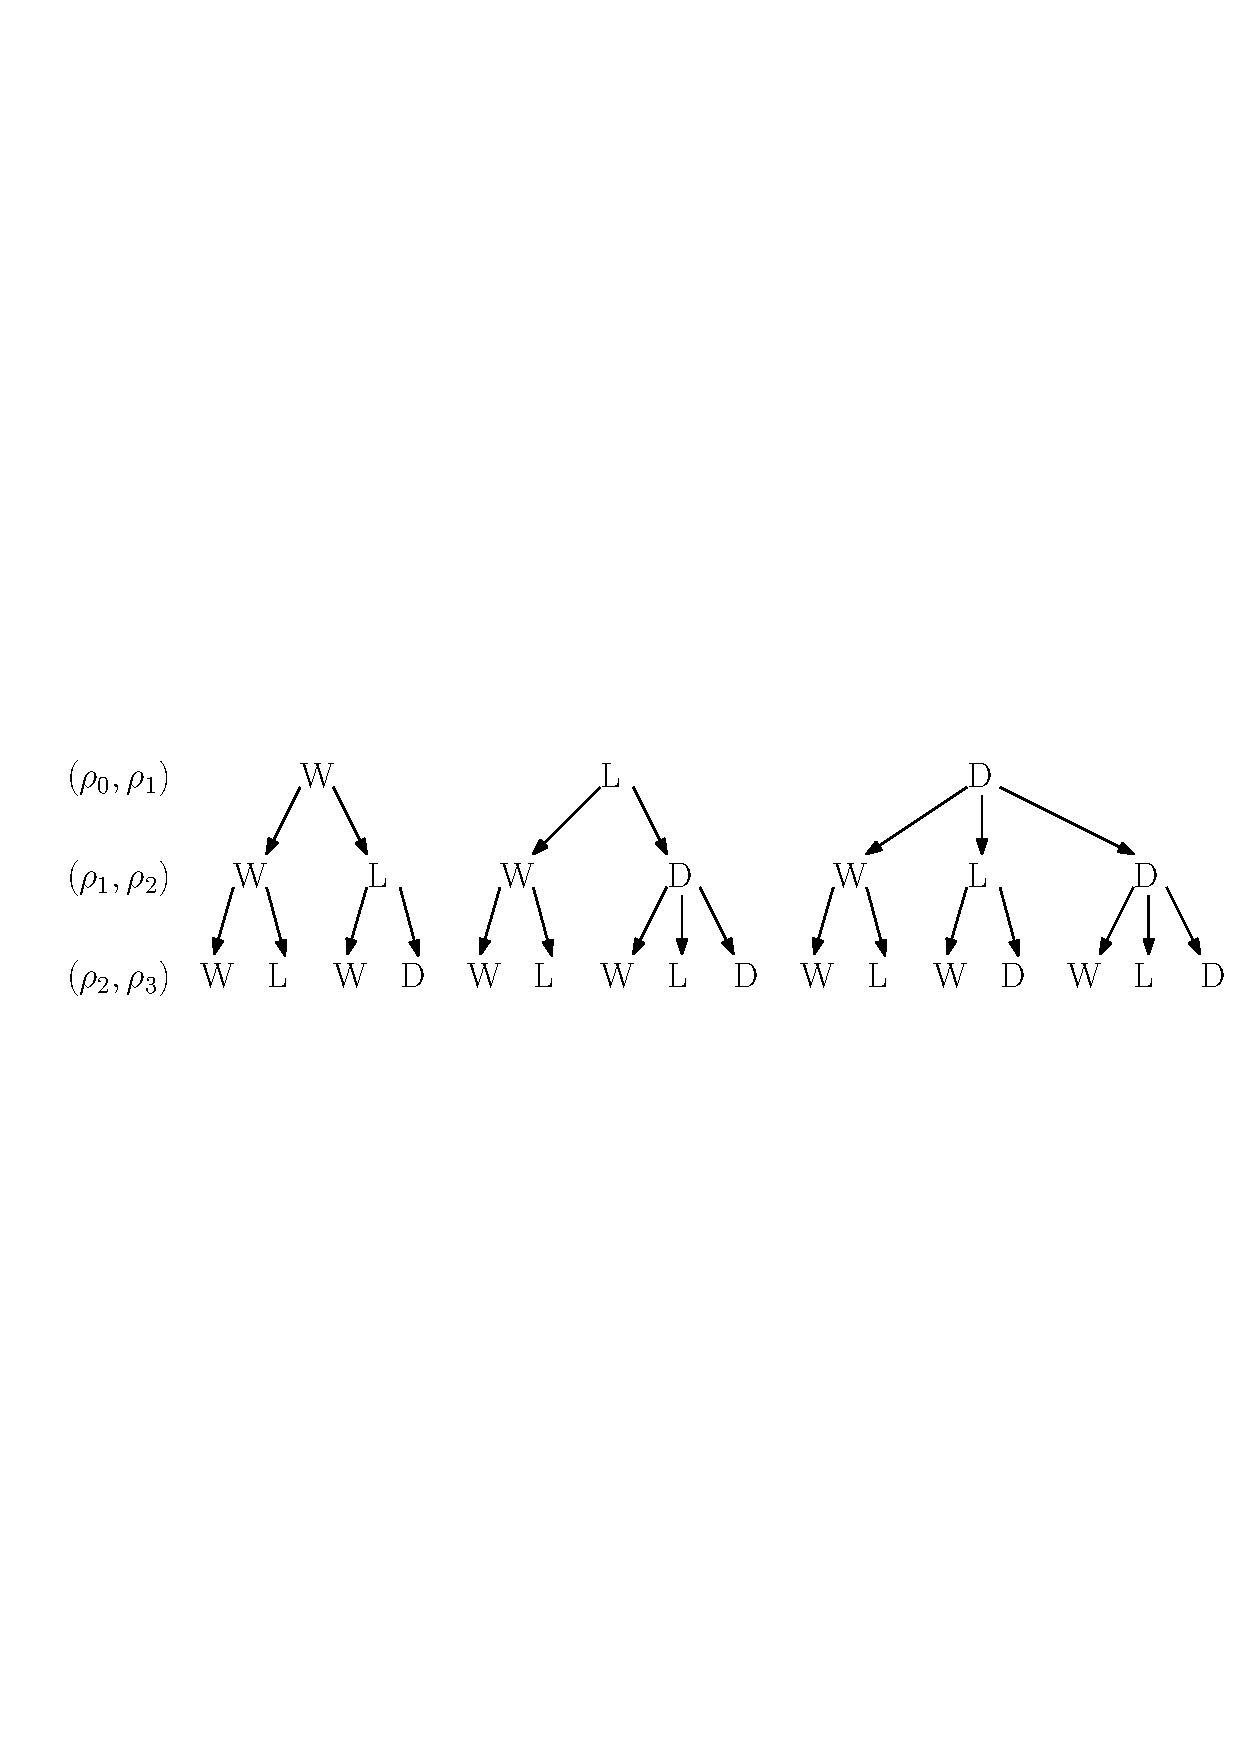
\includegraphics[width=8cm]{figures/threeLevelModes.pdf}
    \caption{The sixteen possible modes for the first three pairs $(\rho_{0},\rho_{1})$, $(\rho_{1},\rho_{2})$, and $(\rho_{2},\rho_{3})$.}
    \label{fig:threeLevelModes}
\end{figure}

We can recursively compute the number of ''modes'' $M_{k}$ with respect to $k$, where $k$ is the number of cells of the discretized link. Let's denote by $w_{k}$, $l_{k}$, and $d_{k}$ the number of modes for which $(\rho_{k},\rho_{k+1})$ is in \textbf{W}, \textbf{L}, and \textbf{D} respectively. Then we have these equations: 

\begin{equation}
w_{0} = l_{0} = d_{0} = 1
\label{eq:modes1}
\end{equation}

\begin{equation}
\begin{array}{lllllll}
w_{k+1} & = & w_{k} & + & l_{k} & + & d_{k}\\
l_{k+1} & = & w_{k} & + & d_{k} & & \\
d_{k+1} & = & l_{k} & + & d_{k} & &
\end{array} \quad \text{for }k \geq 0
\label{eq:modes2}
\end{equation}

\begin{equation}
n_{k} = w_{k} + l_{k} + d_{k} \quad \text{for }k \geq 0
\label{eq:modes3}
\end{equation}

Using matrix notations, equation (\ref{eq:modes2}) reads:

\begin{equation}
\left[ \begin{array}{c}
w_{k+1} \\
l_{k+1} \\
d_{k+1} \end{array} \right] = A \times 
\left[ \begin{array}{c}
w_{k} \\
l_{k} \\
d_{k} \end{array} \right]
\label{eq:modes4}
\end{equation}

\noindent where

\begin{equation}
A = \left[ \begin{array}{ccc}
1 & 1 & 1 \\
1 & 0 & 1 \\
0 & 1 & 1 \end{array} \right]
\label{eq:modes5}
\end{equation}

Then 

\begin{equation}
\left[ \begin{array}{c}
w_{k} \\
l_{k} \\
d_{k} \end{array} \right] = A^{k} \times 
\left[ \begin{array}{c}
w_{0} \\
l_{0} \\
d_{0} \end{array} \right]
\label{eq:modes6}
\end{equation}

It is possible to compute $A^{k}$ explicitly by diagonalizing the matrix $A$, to obtain an explicit expression for $w_{k}$, $l_{k}$, and $d_{k}$ in the form of $a.\beta^{k} + b.\gamma^{k} + c.\delta^{k}$. However, this analytical expression is unwieldy, so we will just derive lower and upper bounds to $n_{k}$. It is easy to see that $d_{k} \leq n_{k}/2$ for $k\geq 0$, then we can prove recursively that $3\cdot2^{k} \leq n_{k} \leq 3\cdot(2.5)^{k}$.

\begin{table}[ht]
\centering % used for centering table
\begin{tabular}{|c|c|c|c|c|c|}
  \hline
 number of cells & 1 & 2 & 5 & 10 & 20\\
  \hline
 number of modes & 7 & 16 & 182 & 10426 & 34206521\\
  \hline
 bound without analysis & 7 & 49 & 16807 & 282475249 & $8\cdot 10^{16}$\\
  \hline
\end{tabular}
\label{table:numModes} % is used to refer this table in the text
\caption{Number of modes for a homogeneous road.}
\end{table}

Even if we have found the minimal polyhedral partition of the space, the number of modes grows exponentially as the number of cells increases, so it is difficult to store all the possible modes. However, at any time step, the mode of each cell can be determined among the 7 possible modes and constructed sequentially building up the general mode of the segment of road.


\subsection{The heterogeneous case}\label{sec:CDFD}

\begin{figure}[ht]
  \centering
    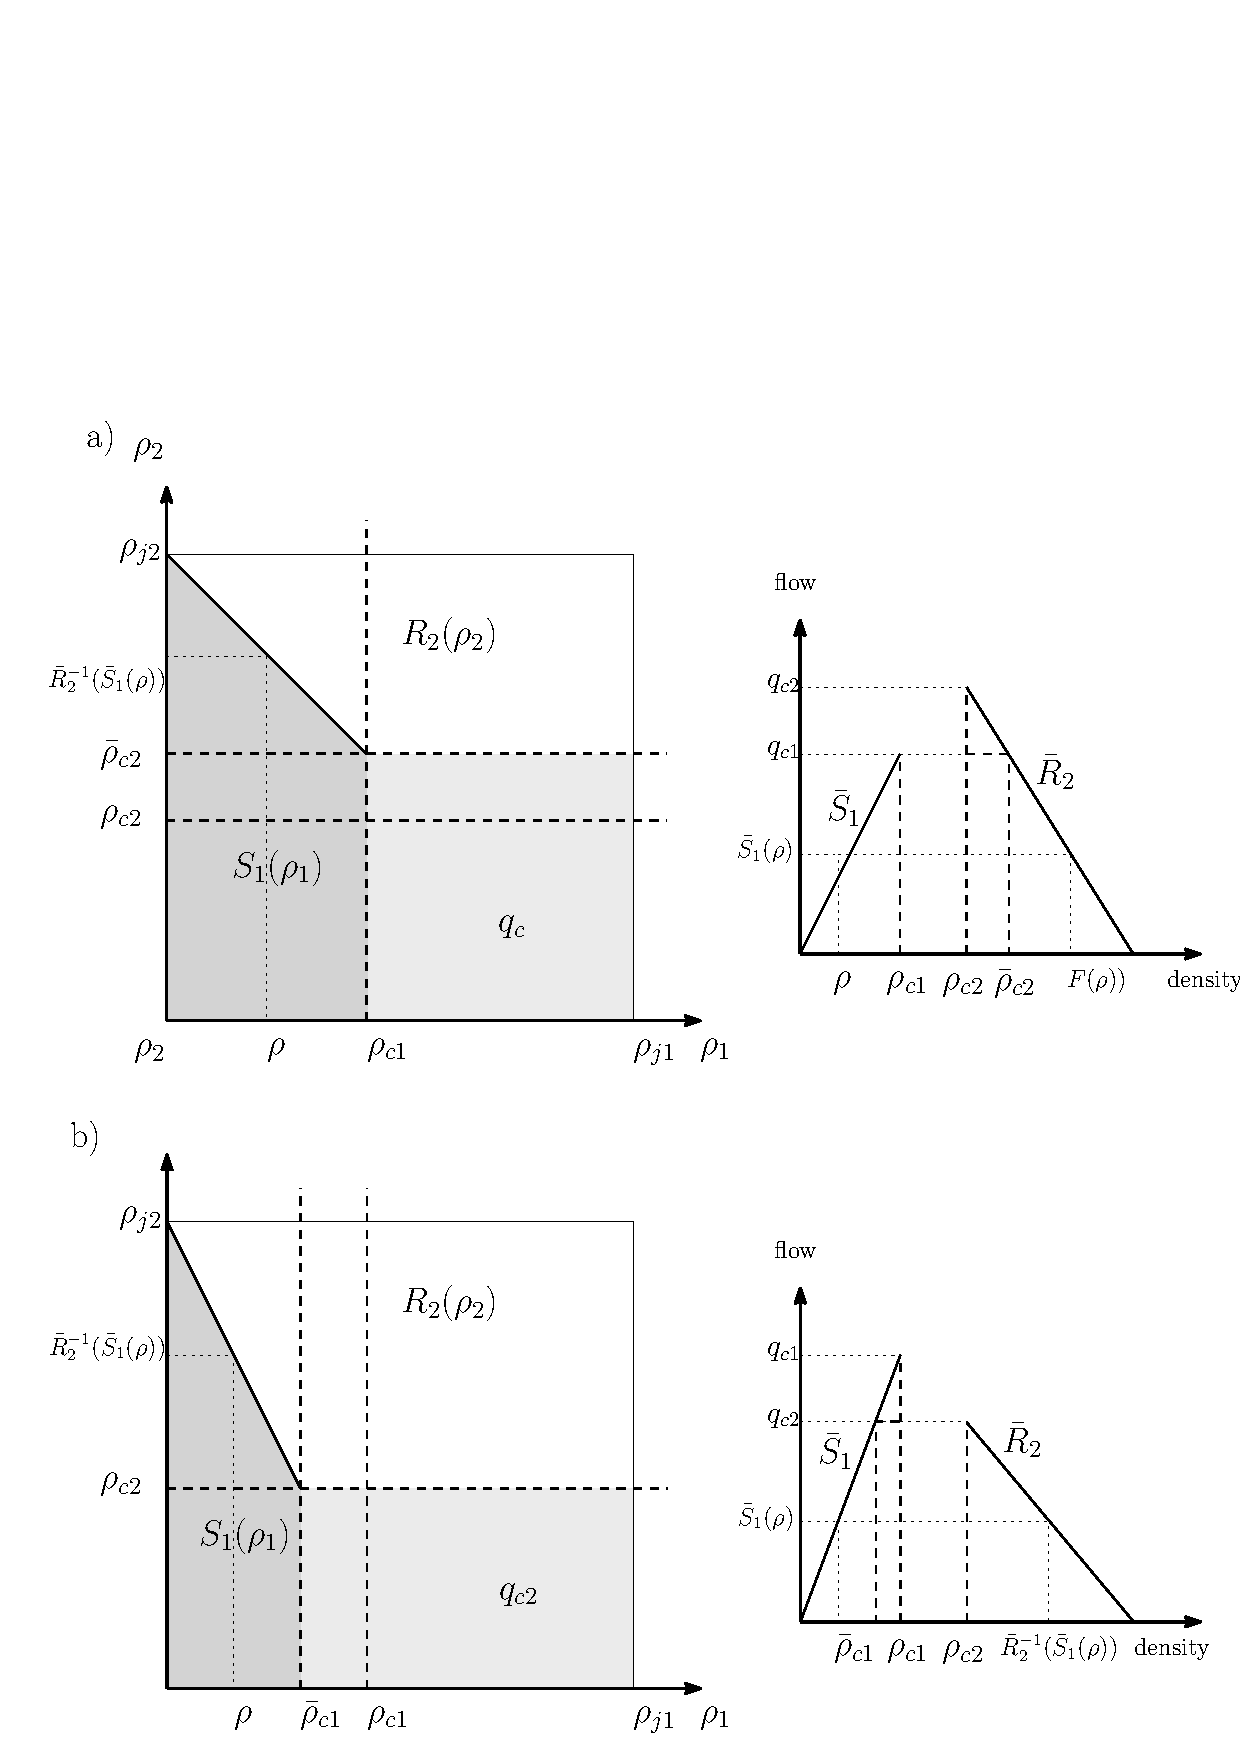
\includegraphics[width=8cm]{figures/godunovDiagram3.pdf}
    \caption{Values of $G(\rho_{1},\rho_{2})$ in the space $(\rho_{1},\rho_{2})$ for the Daganzo-Newell fundamental diagram with different capacities $q_{c1} < q_{c2}$ for a) and $q_{c1} > q_{c2}$ for b). Note that for illustration purposes we suppose $\rho_{c1}\leq\rho_{c2}$.}
    \label{fig:godunovDiagram3}
\end{figure}

In this section, we study the CTM for a heterogeneous road, i.e. $\omega_{f}$, $v_{f}$, $\rho_{j}$, $\rho_{c}$, $q_{c}$ can vary along the link and we add the subscript $i$: $\alpha_{i}$, $\omega_{fi}$, $v_{fi}$, $\rho_{ji}$, $\rho_{ci}$, $q_{ci}$ for the parameters of the fundamental diagram $Q_{i}$ at cell $i$, and the associated sending and receiving flows $S_{i}$, $R_{i}$. Figure \ref{fig:godunovDiagram3} shows the explicit values taken by $G(\rho_{1},\rho_{2})$ in different regions of the space $(\rho_{1},\rho_{2})$ when $q_{c1} < q_{c2}$. We note that the critical density $\rho_{c2}$ is increased to the \textit{effective} critical value $\bar{\rho}_{c2}$ for the receiving flow $R_{2}$, with $\bar{\rho}_{c2} = \bar{R}^{-1}_{2}(q_{c1})$, and the \textit{effective} capacity is $\bar{q}_{c} = q_{c1}$, which is the capacity of the sending flow $S_{1}$. And Figure \ref{fig:godunovDiagram3} also shows the explicit values taken by $G(\rho_{1},\rho_{2})$ in different regions of the space $(\rho_{1},\rho_{2})$ when $q_{c1} > q_{c2}$. Similarly, the critical density $\rho_{c1}$ is decreased to the \textit{effective} value $\bar{\rho}_{c1}$ for the sending flow $S_{1}$ with $\bar{\rho}_{c1} = \bar{S}^{-1}_{1}(q_{c2})$, and the \textit{effective} capacity is $\bar{q}_{c} = q_{c2}$, which is the capacity of the receiving flow $R_{2}$. The Godunov flux has a more general expression \ref{eq:rhoGodunovFlux2}:

\begin{equation}
G(\rho_{1},\rho_{2}) = \begin{cases}
R_{2}(\rho_{2}) & \text{if } (\rho_{1},\rho_{2}) \in \textbf{W}\\
\bar{q}_{c} & \text{if } (\rho_{1},\rho_{2}) \in \textbf{L}\\
S_{1}(\rho_{1}) & \text{if } (\rho_{1},\rho_{2}) \in \textbf{D}
\end{cases}
\label{eq:rhoGodunovFlux2}
\end{equation}

\begin{equation}
\begin{array}{lll}
\textbf{W} & = \{(\rho_{1},\rho_{2}) \mid & \rho_{2} > F(\rho_{1}) \text{ ,   } \rho_{2} > \bar{\rho}_{c2}\}\\
\textbf{L} & = \{(\rho_{1},\rho_{2}) \mid & \rho_{1} > \bar{\rho}_{c1} \text{ ,   } \rho_{2} \leq \bar{\rho}_{c2}\}\\
\textbf{D} & = \{(\rho_{1},\rho_{2}) \mid & \rho_{2} \leq F(\rho_{1}) \text{ ,   } \rho_{1} \leq \bar{\rho}_{c1}\}
\end{array}
\label{eq:regionsHetero}
\end{equation}

\noindent where the boundary between the white and grey regions follows the $(\rho_{1},\rho_{2})=(\rho_{1},F(\rho_{1}))$ trajectory with $F(\rho_{1})= \bar{R}^{-1}_{2}(\bar{S}_{1}(\rho_{1}))$ for $\rho_{1} \leq \rho_{c1}$. $\bar{S}$ and $\bar{R}$ denote the restrictions of the sending and receiving flows to the sub-regions $[0,\rho_{c})$ and $(\rho_{c},\rho_{j}]$ respectively, which also correspond to the left and right parts (w.r.t. $\rho_{c}$) of the fundamental diagram, as shown in the Figure \ref{fig:godunovDiagram3}.

\noindent When the velocity is the Daganzo-Newell function (\ref{eq:dnVelocity}), the Godunov Flux \ref{eq:rhoGodunovFlux2} becomes \ref{eq:rhoGodunovFlux3}:

\begin{equation} \label{eq:rhoGodunovFlux3a}
G_{DN}(\rho_{1},\rho_{2}) = \begin{cases}
-\omega_{f2} \left( \rho_{2} - \rho_{j2} \right) & \text{if } (\rho_{1},\rho_{2}) \in \textbf{W}\\
\bar{q}_{c} & \text{if } (\rho_{1},\rho_{2}) \in \textbf{L}\\
v_{f1} \rho_{1} & \text{if } (\rho_{1},\rho_{2}) \in \textbf{D}
\end{cases}
\end{equation}

\noindent and the boundary between the white and dark-grey regions is:

\begin{equation} \label{eq:boundaryHetero}
(\rho_{1},\rho_{2})=(\rho_{1},-\frac{v_{f1}}{\omega_{f2}}\rho_{1}+\rho_{j2})
\end{equation}

\noindent And \textbf{W}, \textbf{L}, \textbf{D} form a polyhedral partition of the space:

\begin{equation}
\begin{array}{lll}
\textbf{W} & = \{(\rho_{1},\rho_{2}) \mid & \rho_{2} + \frac{v_{f1}}{\omega_{f2}}\rho_{1} > \rho_{j2} \text{ ,   } \rho_{2} > \bar{\rho}_{c2}\}\\
\textbf{L} & = \{(\rho_{1},\rho_{2}) \mid & \rho_{1} > \bar{\rho}_{c1} \text{ ,   } \rho_{2} \leq \bar{\rho}_{c2}\}\\
\textbf{D} & = \{(\rho_{1},\rho_{2}) \mid & \rho_{2} + \frac{v_{f1}}{\omega_{f2}}\rho_{1} \leq \rho_{j2} \text{ ,   } \rho_{1} \leq \bar{\rho}_{c1}\}
\end{array}
\label{eq:regions4}
\end{equation}

At cell $i$, this implies the effective density $\bar{\rho}^{u}_{ci}$ associated with the upstream boundary can be different from the effective density $\bar{\rho}^{d}_{ci}$ associated with the downstream boundary, depending of the capacity drops at these boundaries. Hence, using the notations introduced in section \ref{sec:decompositionModes} all the combinations between $(\rho_{-},\rho)$ and $(\rho,\rho_{+})$ can be possible so we have nine modes. Consequently, for a discretization in $n$ cells, the number of possible modes is $3^{n+1}$.

\begin{table}[ht]
\centering % used for centering table
\begin{tabular}{|c|c|c|c|c|c|}
  \hline
 number of cells & 1 & 2 & 5 & 10 & 20\\
  \hline
 number of modes & 9 & 27 & 729 & 177147 & $10^{10}$\\
  \hline
\end{tabular}
\label{table:numModes2} % is used to refer this table in the text
\caption{Number of modes for a heterogeneous road.}
\end{table}

\begin{comment}

\subsection{Kalman filtering-DRAFT}

and $F_{LH}[.]$, have the same expression with $f_{DN}(.)$ and $f_{LH}(.)$ respectively (as defined in Table. For instance, when we have a Daganzo-Newell fundamental diagram with update operator for the dynamic system $F_{DN}[.]$ (i.e. $\boldsymbol\rho^{t} = F_{DN}[\boldsymbol\rho^{t-1}]$), and suppose that the mode at $x=i$ is three ($m_{i}=3$) then\footnotemark: 

\begin{equation}
F_{i}[\boldsymbol\rho^{t-1}] = f_{DN,m_{i}}(\rho^{t-1}_{i_{-},i,i_{+}}) = f_{DN,3}(\rho^{t-1}_{i_{-},i,i_{+}}) = 
\rho^{t-1}_{i} + \alpha \omega_{f}\rho^{t-1}_{i+1} - \alpha \omega_{f}\rho_{c}
\label{eq:example}
\end{equation}

\footnotetext{
As we have seen earlier, $\alpha$, $\omega_{f}$, $v_{f}$, $\rho_{j}$, $\rho_{c}$, $q_{c}$ can vary along the link and a proper notation would be $\alpha_{i}$, $\omega_{fi}$, $v_{fi}$, $\rho_{ji}$, $\rho_{ci}$, $q_{ci}$ for the parameters of the fundamental diagram at $x=i$, so that:
\[
F_{i}[\rho^{t-1}] = f_{DN,m_{i}}(\rho^{t-1}_{i_{-},i,i_{+}}) = f_{DN,3}(\rho^{t-1}_{i_{-},i,i_{+}}) = 
\rho^{t-1}_{i} + \alpha_{i} \omega_{fi}\rho^{t-1}_{i+1} - \alpha_{i} \omega_{fi}\rho_{ci}
\]
}

In order to use the \textit{Extended Kalman filter} to estimate the state of the link given a sequence of noisy observations, we model the process in accordance with the framework of the \textit{Extended Kalman filter} by adding a white noise to the underlying dynamic system model. The ''true'' state $\boldsymbol\rho^{t}$ is then:

\begin{equation}
\boldsymbol\rho^{t} = F[\boldsymbol\rho^{t-1}] + \boldsymbol\eta^{t}
\label{eq:underlyingSystem3}
\end{equation}

\noindent where $\boldsymbol\eta^{t}\sim N(0,Q_{t})$ is the Gaussian zero-mean, white state noise with covariance $Q_{t}$. The estimated state at time $t$ is denoted by $\hat{\boldsymbol\rho}^{t}$ and the estimated covariance by $P_{t}$. The \textit{prediction step} gives the \textit{a priori} state estimate and covariance $\hat{\boldsymbol\rho}^{t:t-1}$ and $P_{t:t-1}$:

\begin{equation}
\begin{array}{ll}
\text{Predicted state estimate: } & \hat{\boldsymbol\rho}^{t:t-1} = F[\hat{\boldsymbol\rho}^{t-1}]\\
\text{Predicted covariance estimate: } & P_{t:t-1} = F_{t-1}P_{t-1}(F_{t-1})^{T} + Q_{t-1}
\end{array}
\end{equation}

\noindent where $F_{t}$ is the state transition defined to be the following Jacobian:

\begin{equation}
F_{t} = \left(\frac{\partial F_{i}[\rho^{t}]}{\partial \rho^{t}_{j}}\right)_{i,j}
\label{eq:jacobian2}
\end{equation}

The estimated mode $\hat{\boldsymbol m}^{t}$ associated to the estimated vector state $\hat{\rho}^{t}$ is defined from Table \ref{table:modes}. Specifically, in the context of our traffic model, the density at $x=i$ only depends on the densities at the neighbor points $x=i-1,i,i+1$. So $F_{t}$ is a $(n+2)\times(n+2)$ tridiagonal matrix, such that the diagonal elements are $\{0, J_{\hat{m}_{1},2},...,J_{\hat{m}_{n},2},0\}$, the lower diagonal elements are $\{J_{\hat{m}_{1},1},J_{\hat{m}_{2},1},...,J_{\hat{m}_{n},1},0\}$, and the upper diagonal elements are $\{0,J_{\hat{m}_{1},3},J_{\hat{m}_{2},3},...,J_{\hat{m}_{n},3}\}$, where $J$ is defined in Equation \ref{eq:jacobian}. 

In the case of the Daganzo-Newell fundamental diagram, the operator $F_{DN}[.]$ defined in (\ref{eq:underlyingSystem2}) is \textit{linear} (from the linearity of $f_{DN}$). Along with the assumption of a white state noise, the \textit{prediction step} (\ref{eq:predict}) of the \textit{Extended Kalman filter} is actually identical to the regular \textit{Kalman filter}, and it is known from the theory that the \textit{Kalman filter} is optimal \cite{Anderson2005}.

In the case of a linear-hyperbolic velocity function, the operator $F_{LH}[.]$ is not linear if at some points of the discrete space the mode is between four and seven. Then the \textit{Extended Kalman filter} is \textit{near-optimal}.

We can note that the first line and first column of $P_{t}$ have only zero elements because the boundary condition $\rho^{t}_{0}$ is deterministic (i.e. $cov(\rho^{t}_{0},\rho^{t}_{i})=0$ for $i=1,...,n$), and similarly the last line and last column of $P_{t}$ are null since the boundary condition $\rho^{t}_{n+1}$ is deteministic. Additionally, the observation model for the link is given by:

\begin{equation}
\boldsymbol y^{t} = H_{t}\boldsymbol\rho^{t} + \boldsymbol\chi^{t}
\end{equation}

\noindent where $H_{t}\in \{ 0,1 \}^{p_{t}\times n}$ is the linear observation observation matrix which encodes the $p_{t}$ observations (each one of them being at a discrete cell on the highway) for which the density is observed during discrete time step $t$, and $n$ is the number of cells along the link. The last term in (\ref{eq:observation}) is the white, zero mean observation noise $\boldsymbol\chi^{t} \sim N(0,R_{t})$ with covariance matrix $R_{t}$. The \textit{update step} is:

\begin{equation}
\begin{array}{ll}
\text{Kalman gain: } & K_{t} = P_{t:t-1}H_{t}^{T}\left(H_{t}P_{t:t-1}H_{t}^{T}+R_{t}\right)^{-1}\\
\text{Updated state estimate: } & \hat{\boldsymbol\rho}^{t} = \hat{\boldsymbol\rho}^{t:t-1} + K_{t}(\boldsymbol y^{t} - H_{t}\hat{\boldsymbol\rho}^{t:t-1})\\
\text{Updated estimate covariance: } & P_{t} = (I - K_{t}H_{t})P_{t:t-1}
\end{array}
\end{equation}

The Extended Kalman filter provides the distribution of $\hat{\boldsymbol\rho}^{t}$ given the sequence of observations $\boldsymbol y^{0:t}$, sequence of modes $\hat{\boldsymbol m}^{0:t} = \{\hat{\boldsymbol m}^{0},...,\hat{\boldsymbol m}^{t}\}$, and sequence of control parameters $\boldsymbol u^{0:t}$, which is exactly equal to the distribution of $\hat{\boldsymbol\rho}^{t}$ since the sequence $\hat{\boldsymbol m}^{0:t}$ is deterministic. Concretely, the vector of control parameters $\boldsymbol u^{t}$ contain the vector of critical densities $\boldsymbol\rho_{c}$, the vector of jam densities $\boldsymbol\rho_{j}$, and the boundary conditions $\rho^{t}_{0}$ and $\rho^{t}_{n+1}$. Theoretically, the result is obtained by marginalizing the joint distribution of $\hat{\boldsymbol\rho}^{t}$ and $\hat{\boldsymbol m}^{0:t}$ as follows:

\begin{equation}
\begin{array}{ll}
p(\hat{\boldsymbol\rho}^{t}|\boldsymbol y^{0:t},\boldsymbol u_{0:t}) & =
\int_{\mathcal{M}_{n}} p(\hat{\boldsymbol\rho}^{t}|\boldsymbol y^{0:t},\boldsymbol u^{0:t},\boldsymbol m^{0:t})p(\boldsymbol m^{0:t}|\boldsymbol y^{0:t},\boldsymbol u^{0:t})
d\boldsymbol m^{0:t}\\ 
& = \int_{\mathcal{M}_{n}} p(\hat{\boldsymbol\rho}^{t}|\boldsymbol y^{0:t},\boldsymbol u^{0:t},\boldsymbol m^{0:t})\boldsymbol 1_{\hat{\boldsymbol m}^{0:t}}d\boldsymbol m^{0:t}\\[1ex]
& = p(\hat{\boldsymbol\rho}^{t}|\boldsymbol y^{0:t},\boldsymbol u^{0:t},\hat{\boldsymbol m}^{0:t})
\label{eq:marginalization}
\end{array}
\end{equation}

\subsection{Implementation-DRAFT}

\subsubsection{Algorithm for the \textit{prediction step}}

Algorithm using the structure of $F_{t}$ and extension to a network

From Appendix \ref{sec:modes},  In (\ref{eq:predict}), the \textit{a priori} state estimate $\hat{\boldsymbol\rho}^{t:t-1}$ is derived through the algorithm in (\ref{eq:underlyingSystem2}).

\subsubsection{Accuracy}

For a Daganzo-Newell fundamental diagram, we can note that the decomposition in different modes in (\ref{eq:underlyingSystem2}) is in fact a special case of \textit{Conditional Dynamic Linear Model} (CDLM) as described in \cite{Chen2000} with a discrete latent indicator that is deterministic. In this case, there is only one estimated deterministic sequence of modes $\hat{\boldsymbol m}^{0:t}$ or latent indicators, hence there is no need to use a sequential Monte-Carlo method to sample an ensemble of trajectories of modes. The Mixture Kalman Filter \cite{Chen2000} reduces to a simple Kalman Filter. For non-triangular fundamental diagrams which have the characteristics \textbf{LWR1-6}, a first order Taylor Series expansion is applied. Such a linearization is a good approximation. Then the Extended Kalman filter can be applied to each mode.

In our case, the estimated sequence of modes $\hat{\boldsymbol m}^{0:t}$ is readily infered through the Godunov scheme, and at all the cells along the link, including those where there is no observation. Contrary to some previous models as in \cite{Munoz2003}, the modes are not directly sampled from density measurements along the highway. However, the mode is still indirectly infered from those measurements by assimilating the observations with the \textit{update state} of the Kalman filter. Besides, we rely on the accuracy of the estimation of the mode provided by the Godunov scheme when we apply the Kalman filter for each mode. Such an assumption that favors the mode provided by the Godunov scheme is yet another reason why the sequential Monte-Carlo method (with the resampling step) is not used in the algorithm, because we then suppose that our sequence of modes is the one with the largest likelihoods. (to develop, do a test of likelihood)

\subsubsection{Complexity}

Comparison with the Extended Kalman filter and matlab simulations and results

\end{comment}